\documentclass{beamer}
%
% Choose how your presentation looks.
%
% For more themes, color themes and font themes, see:
% http://deic.uab.es/~iblanes/beamer_gallery/index_by_theme.html
%
\mode<presentation>
{
  \usetheme{Darmstadt}      % or try Darmstadt, Madrid, Warsaw, ...
  \usecolortheme{crane} % or try albatross, beaver, crane, ...
  \usefonttheme{default}  % or try serif, structurebold, ...
  \setbeamertemplate{navigation symbols}{}
  \setbeamertemplate{caption}[numbered]
}

\usepackage[T1]{fontenc}
\usepackage{hyperref}
\usepackage{color}
\usepackage[english]{babel}
\usepackage[utf8x]{inputenc}
\usepackage{centernot}
\usepackage{verbatim}
%\usepackage[final]{pdfpages}

\hypersetup{
  colorlinks, linkcolor=blue
}

\title[Java lists, maps and not only]{Java lists, maps and not only\ldots}
\author{Paweł Jaworski}
\institute{Luxoft Poland Sp. z o.o.}
%\date{2014-06-09}
\date{2019-10-22}

\begin{document}

\begin{frame}
  \titlepage
\end{frame}

\begin{frame}{Outline}
  \tableofcontents
\end{frame}

\section{Lists}

\begin{frame}{Introduction}

\begin{itemize}
  \item Java collections are sophisticated implementations of algorithms for storing data (see also Cormen's ``Introduction to algorithms'')
  \item All collections implement iteration
  \item Lists are implemented as sequential collections backed by arrays and linked lists
  \item Sets, besides iteration, are also allowing checking if the item is present.
  \item Maps are associative containers which allow quick access by object-key (any object, also other than integer).
  \item Trees are underlying some implementations of Maps and Sets
  \item Lists maintain item order while it is not guaranteed in Sets and Maps.
\end{itemize}

\end{frame}

\begin{frame}{The plan}
    \begin{figure}[htbp]
    \centering
        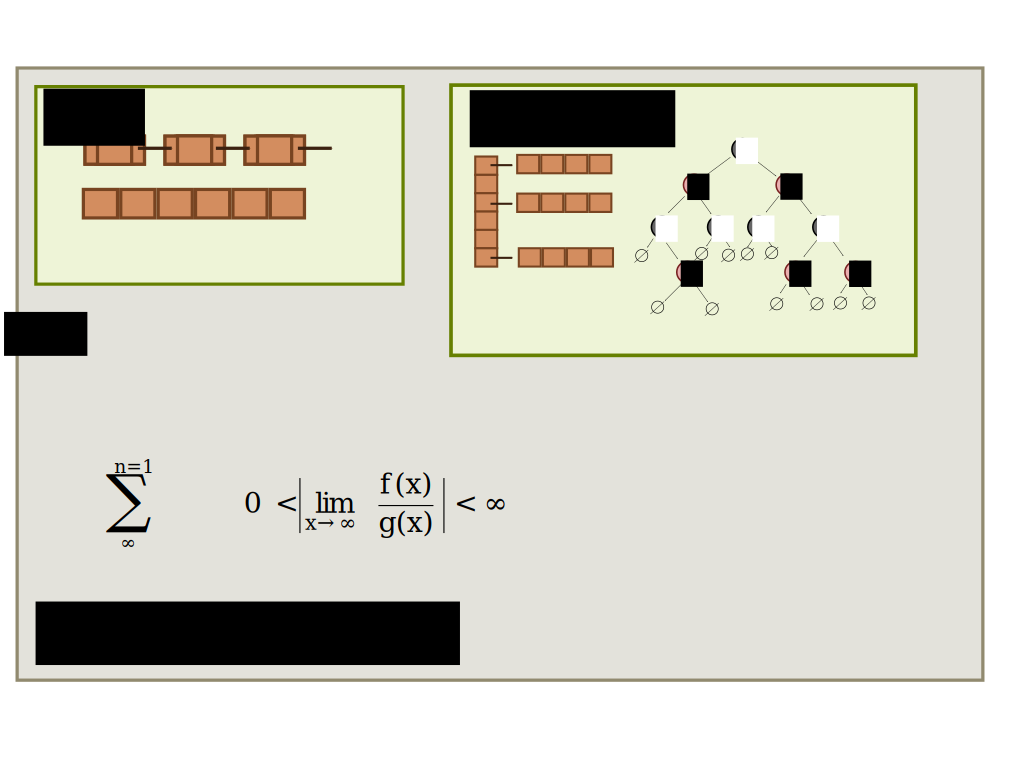
\includegraphics[width=1.00\textwidth]{lab-plan.pdf}
    \caption{Title}
    \label{fig:lab-plan}
    \end{figure}

\end{frame}

\section{Algorithmics}

\subsection{Complexity calculation and nomenclature}

\begin{frame}{The Big O, $\Omega$, $\Theta$ notation}

When there exists $n_0>0$ and $c>0$ for which we can say that:
$$\forall{n>n_0} \; f(n) \leq c\cdot g(n) $$
we say that $f$ is big-O $g$ and write $f(x)=O(g(x))$

When there exists $n_0>0$ and $c>0$ for which we can say that:
$$\forall{n>n_0} \; f(n) \geq c\cdot g(n) $$
we say that $f$ is big-$\Omega$ $g$ and write $f(x)=\Omega(g(x))$


\end{frame}

\begin{frame}{The Big $\Theta$ notation}

When we can say that $f(x)=O(g(x)) \wedge f(x)=\Omega(g(x))$ we say that $f$ is Big $\Theta$ $g$ and write:
$$f(x)=\Theta(g(x))$$

\end{frame}


\begin{frame}{Examples}

\begin{itemize}
	\item Given $g(x)=x^2$ and $f(x)=3x^2+4$ we can say that $f(x)=O(g(x))$.\ldots
	\item Given $g(x)=x^3$ and $f(x)=100x^2+4x^3$ we can say that $f(x)=O(g(x))$.\ldots
    \item Given $g(x)=2^x$ and $f(x)=2^x+x^{64}$ we can say that $f(x)=O(g(x))$.\ldots
\end{itemize}
We can also easily say that $x^2=O(2^x)$, and $x^2=\Omega(1)$ but it is not very interesting. This observation is very weak. We are rather interested in finding the closest matches.

\end{frame}


\begin{frame}{$\Theta$ sufficient condition}
The most interesting is finding the simple in form, but exact, match of the function. This match is symbolised by $\Theta$. $$f(x)=O(g(x)) \wedge f(x)=o(g(x)) \Longrightarrow f(x)=\Theta(g(x))$$

If $f(x)=\Theta(g(x))$, it means that $f$ is grows asymptotically as fast as $g$.

Sufficient condition for $f(x)=\Theta(g(x))$ is:

$$0<\lim_{x\rightarrow\infty}\left\lvert\frac{f(x)}{g(x)}\right\rvert< \infty$$

\end{frame}

\begin{frame}{Some things that programmers usually know}

We use given notation extensively to describe algorithm time of execution (and memory consumption). Hence for us (generally):

\begin{itemize}
	\item $x^2$ is worse than $x$
    \item $x$ is worse than $\log x$
    \item $2^x$ is worse than $x^{16}$ and it's bad
    \item $x!$ -- it's so much, we don't distinguish between $x!$ and $2^x$. Those are equally BAD.
    \item We often don't distinguish between logarithm and exponential bases
\end{itemize}

\end{frame}

\begin{frame}{Examples}
    \begin{figure}[htbp]
    \centering
        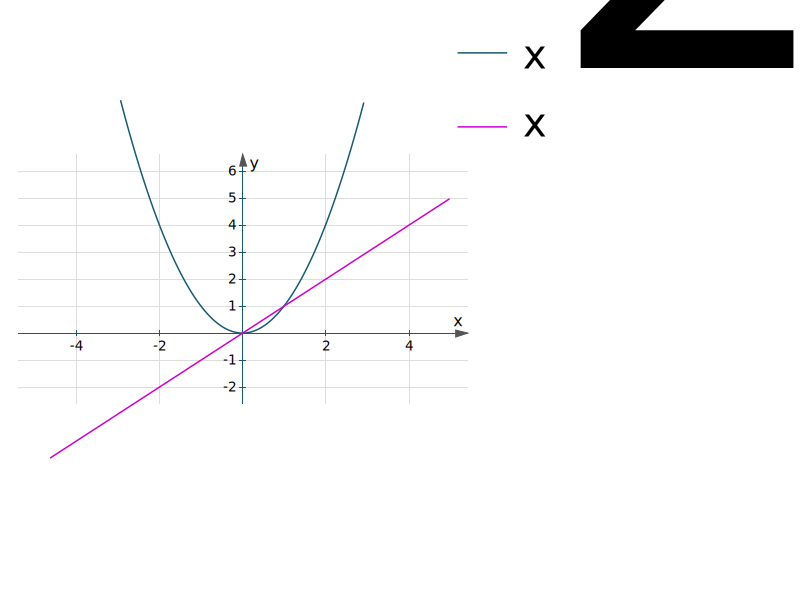
\includegraphics[width=1.00\textwidth]{x2_vs_x.pdf}
    \caption{Title}
    \label{fig:x2_vs_x}
    \end{figure}
\end{frame}

\begin{frame}{Examples}
    \begin{figure}[htbp]
    \centering
        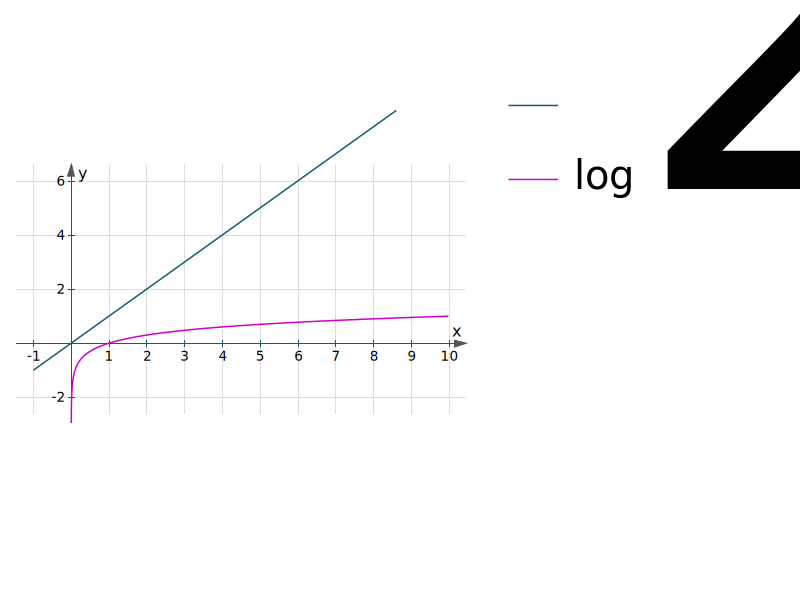
\includegraphics[width=1.00\textwidth]{x_vs_logx.pdf}
    \caption{Title}
    \label{fig:x_vs_logx}
    \end{figure}
\end{frame}

\begin{frame}{Examples}
    \begin{figure}[htbp]
    \centering
        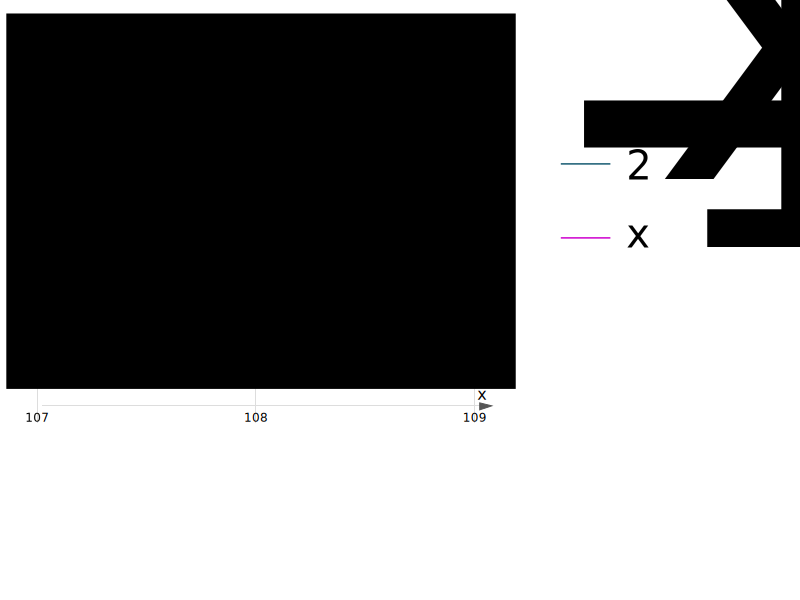
\includegraphics[width=1.00\textwidth]{2pow_x_vs_xpow_16.pdf}
    \caption{Title}
    \label{fig:2powx_vs_xpow16}
    \end{figure}
\end{frame}

\begin{frame}{Worst case scenario}
Programmers also consider worst case (pessimistic) scenarios of algorithms and their complexity. Some algorithms work very slow on some special cases of input data. E.g. \textbf{quicksort}, despite of being $O(n\cdot\textrm{log}n)$ runs at $n^2$ time, when in every partitioning selected pivot divides data to lengths: $1$ and rest.

Having that in mind, we can select, for example, \textbf{heapsort}, which has worst case running time still $n\cdot\textrm{log}n$
\end{frame}

\section{List}

\subsection{ArrayList}

\begin{frame}{Need to know by heart}

\begin{itemize}
\item \textsl{All arrays and lists in Java are indexed from 0!!!}
\end{itemize}

\end{frame}

\begin{frame}{ArrayList}

\begin{itemize}
\item Allocated as a one block in memory (more ``array-ish'' than ``list-ish'')
\item Quick ``please get me an element at position $n$'' (further referred to as \textbf{get}): $\Theta(1)$
\item Slow ``please insert element at position $n$, moving all following elements to the right'' (further referred to as \textbf{insert}): $O(n)$
\item Slow ``please delete element at position $n$, moving all following elements to the left'' (further referred to as \textbf{delete}): $O(n)$
\end{itemize}

\end{frame}

\begin{frame}{ArrayList}

\begin{itemize}
\item Quick \textbf{append} - a special-case of the insert at the last place, i.e. when for $n$ equal number of elements: $\Theta(1)$, but only when the underlying array size is $N>n+1$
\item When ArrayList is full, to perform insert we need to expand underlying array. We do it by increasing size by twice the current size.
\item Is really the \textbf{append} operation $\Theta(1)$???

\end{itemize}

\end{frame}

\begin{frame}{ArrayList pros and cons}
    \begin{itemize}
        \item Insert at an arbitrary place costs $n$ operations for $n=s-i$ where $s$ is number of items and $i$ is the position we insert at.
    \end{itemize}
    \begin{figure}[htbp]
    \centering
        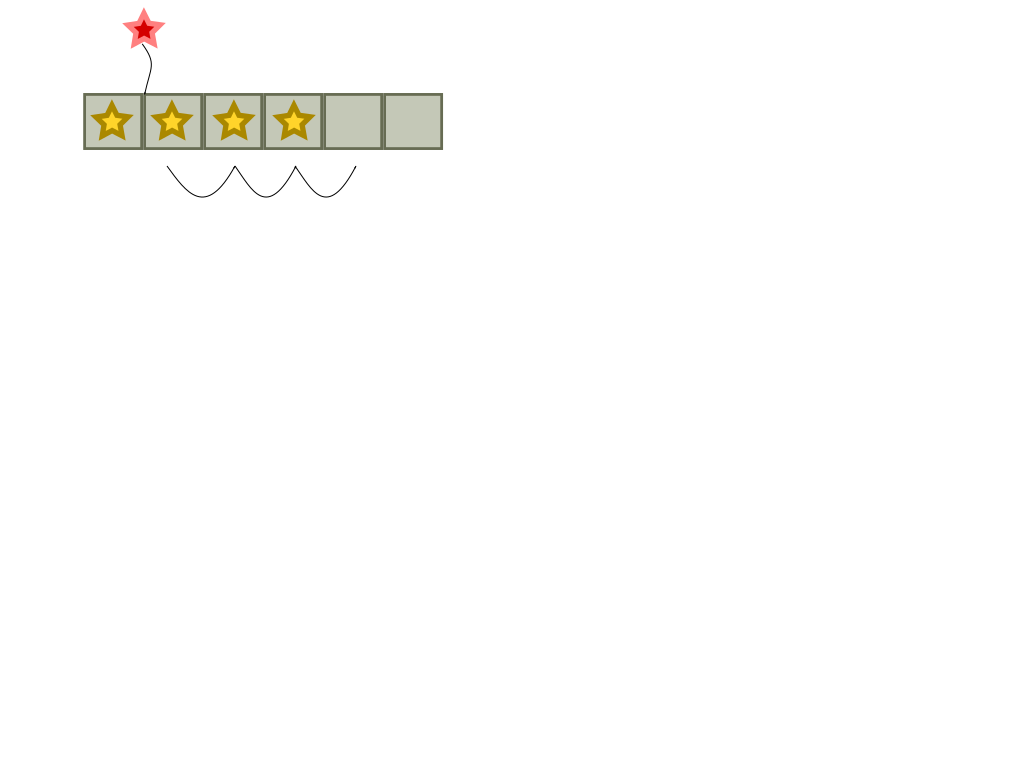
\includegraphics[width=1\textwidth]{insert-list.pdf}
    \label{fig:insert-list}
    \end{figure}
\end{frame}

\begin{frame}{Amortised cost. Amortised analysis}

\begin{itemize}
\item We analyse amortised cost of operations amortised by their number.
\item Amortised cost for given $f(n)$ is $F(n)$ that: $$F(n)=\frac{T(n)}{n}$$
where
$$T(n)=\sum_{x=0}^{n}f(x)$$
\end{itemize}

\end{frame}

\begin{frame}{Amortised cost. Amortised analysis}

\begin{itemize}
\item For array initialised to 2, in the \textbf{append} operation we have cost:
$$1,1,n_1=2,1,1,n_2=4,1,1,1,1,n_3=8$$
where $n_x$ is n-th resize cost equals array's size at the moment of resize.
\item If we use an accounting method to tell that every operation, we put additional 2 operations' time on a special account, for a later use, we can reuse that time at critical sections of resizing. Our account state is then:
\end{itemize}

\end{frame}

\begin{frame}{Amortised cost. Amortised analysis}

\begin{table}
\centering
\begin{tabular}{r|r}
Operation & Account state \\\hline
+2 & 2 \\
+2 & 4 \\
-2 & 2 \\
+2 & 4 \\
+2 & 6 \\
-4 & 2 \\
+2 & 4 \\
+2 & 6 \\
+2 & 8 \\
+2 & 10 \\
-8 & 2 \\\hline
\end{tabular}
\caption{\label{tab:widgets}Amortised analysis using accounting method}
\end{table}

\end{frame}

\begin{frame}{Amortised cost. Amortised analysis}
\begin{center}
    SVG Animation for the amortised cost accounting method
\end{center}
\end{frame}

\begin{frame}{Amortised cost. Amortised analysis}

\begin{itemize}
\item In this case we say that operation \textbf{append} on ArrayList is $O(1)$ and keep in mind that sometimes it can stop our system for a very long time. So if we want to get overall computation time fit, we can allow us to expand a very large ArrayList, but when we are low-latency needers, we might need to search for a better solution.
\end{itemize}

\end{frame}


\subsection{LinkedList}

\begin{frame}{LinkedList}

\begin{itemize}
\item Allocated as linked list of many objects
\item Every inserted object needs a wrapper object, so the number of objects in memory are at least \textbf{twice} the number of elements in list.
\item Fast \textbf{append}: $\Theta(1)$
\item Fast \textbf{insert} but only when given a \textbf{preceeding node} in the list.
\item Fast \textbf{delete} but under the same conditions as \textbf{insert}
\item Slow \textbf{get}: $O(n)$
\item Does not need to grow - \textbf{append} is not lagging from time to time.
\end{itemize}

\end{frame}

\begin{frame}{LinkedList - pros}

\begin{itemize}
\item LinkedList implements \texttt{Deque} which gives us nice stack and fifo methods:
 \texttt{pollFirst}, \texttt{pollLast}, \texttt{peekFirst}, \texttt{peekLast}
\end{itemize}

\end{frame}

\begin{frame}{LinkedList - cons}

\begin{itemize}
\item Every item in LinkedList is of a class LinkedList.Item which has much overhead.
\end{itemize}
    \begin{figure}[htbp]
    \centering
        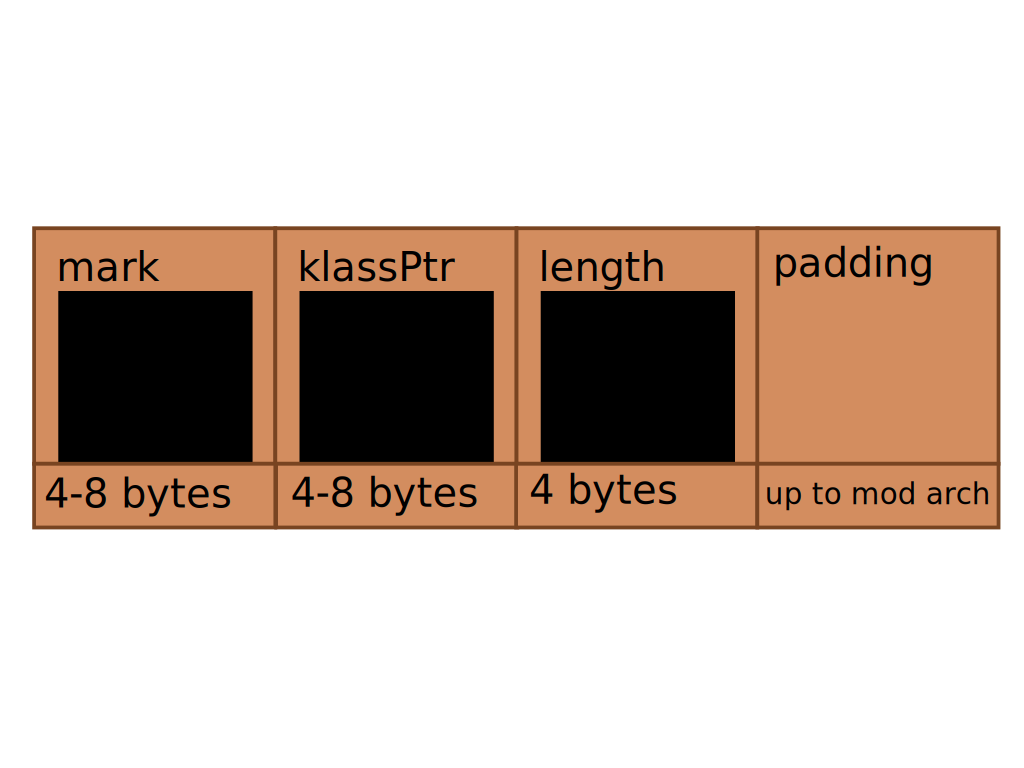
\includegraphics[width=1.00\textwidth]{lab-class-size.pdf}
    \caption{Title}
    \label{fig:lab-class-size}
    \end{figure}
\end{frame}

\begin{frame}[fragile]{How much do the object weight in Java}
    \begin{verbatim}
class A \{ \} \\
\ \\
class B extends A \{ \} \\
\ \\
class C \{ \\
\ \ \ \ boolean a; \\
\}
    \end{verbatim}
\end{frame}

\begin{frame}[fragile]{How much do the object weight in Java - compressed pointers}
\textit{java -XX:+UseCompressedOops}
    \begin{verbatim}
sizeof A = 16 \\
sizeof B = 16 \\
sizeof C = 16 \\
sizeof Boolean = 16 \\
sizeof Char = 16 \\
sizeof Integer = 16 \\
sizeof Long = 24 \\
sizeof class java.util.LinkedList\$Node = 24 \\
    \end{verbatim}
\end{frame}

\begin{frame}[fragile]{How much do the object weight in Java - \textit{not} compressed pointers}
\textit{java -XX:-UseCompressedOops}
\begin{verbatim}
sizeof A = 16 \\
sizeof B = 16 \\
sizeof C = 24 \\
sizeof Boolean = 24 \\
sizeof Char = 24 \\
sizeof Integer = 24 \\
sizeof Long = 24 \\
sizeof class java.util.LinkedList\$Node = 40 \\
\end{verbatim}
\end{frame}

\section{Maps}
\subsection{HashMap}
\begin{frame}{HashMap}

\begin{itemize}
	\item Fast finding element by the key (further referred to as: \textbf{lookup}): $O(1)$.\footnote{When time is longer, in properly setup map (i.e. number of buckets $>$ size), it means that collisions occur. This can be the sign of incorrect hash function.}
    \item Fast putting a key-value pair (further referred to as: \textbf{insert}): $(O(1)$, pessimitically $n=\textrm{size}$, when map needs to grow.
    \item Fast remove: $O(1)$ (HashMap does not shrink).
    \item Values with the same hash stored in $LinkedList$, collisions may occur.
\end{itemize}
\end{frame}

\begin{frame}{HashMap}

\begin{center}x.equals(y) $\Longrightarrow$ x.hashCode() == y.hashCode()\end{center}
\begin{center}x.hashCode() == y.hashCode()  $\centernot\Longrightarrow$ x.equals(y)\end{center}
\end{frame}


\begin{frame}{TreeMap}

\begin{itemize}
	\item Implemented by Red-Black tree.
    \item Keys are sorted.
    \item Quite good lookup: $O(\textrm{log}n)$
    \item Quite good insert: $O(\textrm{log}n)$
    \item Quite good delete: $O(\textrm{log}n)$
    \item Memory consumption: $O(n)$.
\end{itemize}
\end{frame}


\begin{frame}{Red-black tree}
    For each path count of black nodes (``black length'') is constant
    \begin{figure}[htbp]
    \centering
        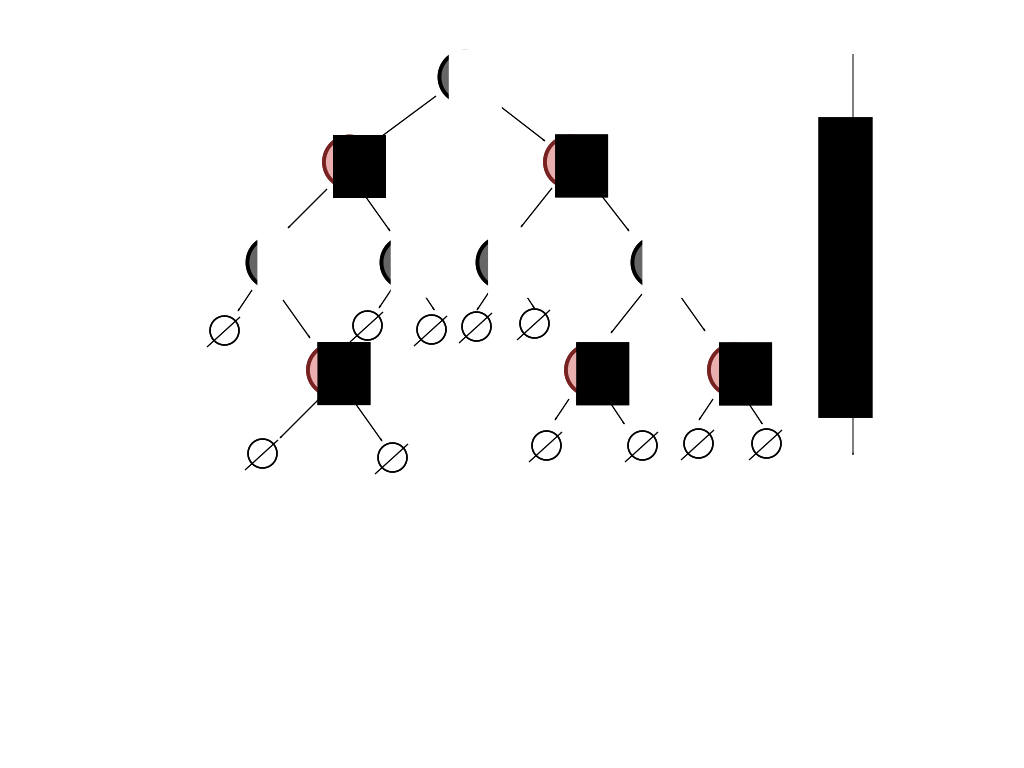
\includegraphics[width=1.00\textwidth]{lab-red-black-tree.pdf}
    \caption{Title}
    \label{fig:lab_red_black_tree}
    \end{figure}

\end{frame}

\begin{frame}{Algorithms visualised}
\begin{center}
    \url{https://www.cs.usfca.edu/~galles/visualization/java/visualization.html}
\end{center}
\end{frame}

\section{Excercises}
\subsection{Laboratory excercises descriptions}


\begin{frame}{Excercise 1}

\begin{itemize}
	\item Open the project, and enter the t1 package
    \item in \texttt{src/\textit{main}/java/t1} we have code that we need to fix
    \item in \texttt{src/\textit{test}/java/t1} we have tests that need to pass
    \item Please implement FIFOQueue using appropriate Java's list implementation
    \item Please implement LIFOQueue using appropriate Java's list implementation
    \item What happens when we change the selected implementation of list to another? Does the test still pass? What is the difference
\end{itemize}
\end{frame}

\begin{frame}{Excercise 2}

\begin{itemize}
    \item see \texttt{src/\textit{main}/java/t2} and \texttt{src/\textit{test}/java/t2}
    \item First ocus on \texttt{first\_exercise\_testGBPtoPLN}
    \item why there is no such currency conversion, providing that we have added it in the map in \texttt{initStatic()} method?
    \item Next focus on \texttt{second\_excercise\_testPLNtoGBP}
    \item Why the test is failing? What is the printed result?
\end{itemize}
\end{frame}

\begin{frame}{Excercise 3}

\begin{itemize}
    \item see \texttt{src/\textit{main}/java/t3} and \texttt{src/\textit{test}/java/t3}
    \item List must not grow, must throw proper exceptions.
    \item List must contain the java's Array as as storage for the items
    \item How to initialize the storing array for any T? Why \texttt{new T[]} is not working?
\end{itemize}
\end{frame}

\begin{frame}{Excercise 4}

\begin{itemize}
    \item see \texttt{src/\textit{main}/java/t4} and \texttt{src/\textit{test}/java/t4}
    \item Why the assertNull does not work?
\end{itemize}
\end{frame}

\begin{frame}{Excercise 5}

\begin{itemize}
    \item see \texttt{src/\textit{main}/java/t5} and \texttt{src/\textit{test}/java/t5}
    \item Uncomment code in the test
    \item Why the code does not compile? How can we fix it?
\end{itemize}
    \begin{figure}[htbp]
    \centering
        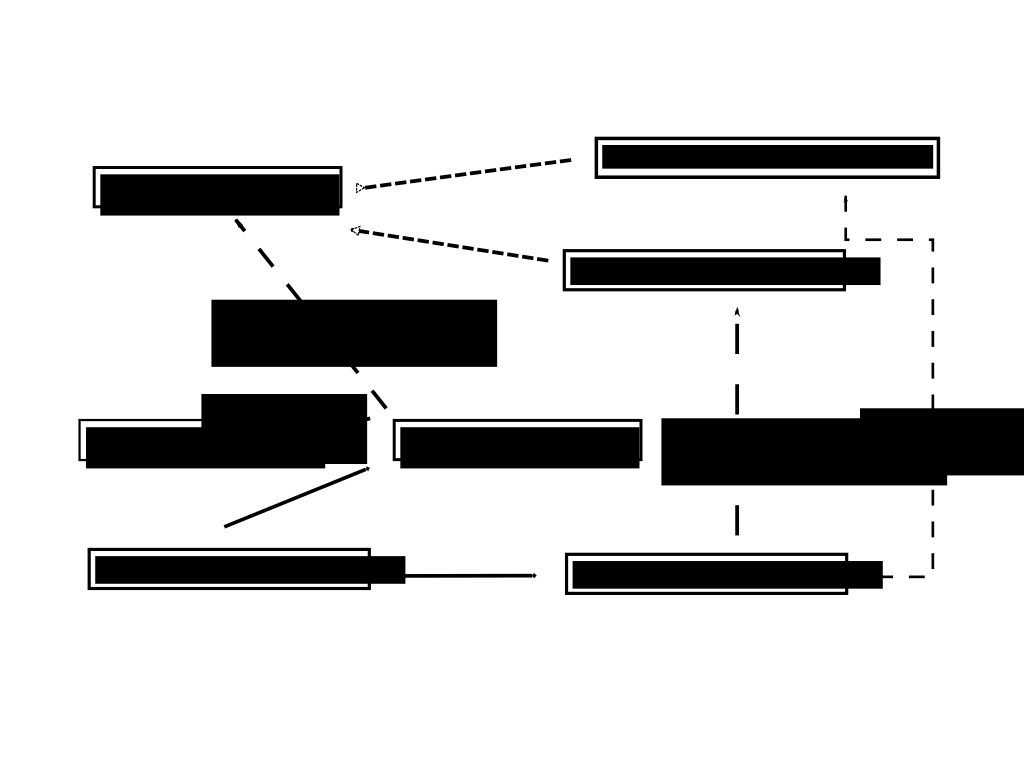
\includegraphics[width=0.9\textwidth]{t5-uml.pdf}
    \label{fig:t5-uml}
    \end{figure}
\end{frame}

\begin{frame}{Excercise 6}

\begin{itemize}
    \item see \texttt{src/\textit{main}/java/t6} and \texttt{src/\textit{test}/java/t6}
    \item \texttt{testRunningTimeEasy} - focus on time of execution, why it is so slow
    \item \texttt{testMemEfficiencyEasy} - focus on time of execution, why it is so slow
\end{itemize}
\end{frame}

\section{Summary}
\subsection{What have we learned today?}
\begin{frame}{HashMap}

    \begin{itemize}
        \item Test Driven Development.
        \begin{itemize}
            \item Always start with test \pause
            \item Test must fail \pause
            \item Make the test passing by fixing the code \pause
        \end{itemize}
        \item Fast putting a key-value pair (further referred to as: \textbf{insert}): $(O(1)$, pessimitically $n=\textrm{size}$, when map needs to grow.
        \item Fast remove: $O(1)$ (HashMap does not shrink).
        \item Values with the same hash stored in $LinkedList$, collisions may occur.
    \end{itemize}
\end{frame}


% \subsection{Mathematics}

% \begin{frame}{Readable Mathematics}

% % Commands to include a figure:
% %\begin{figure}
% %\includegraphics[width=\textwidth]{your-figure's-file-name}
% %\caption{\label{fig:your-figure}Caption goes here.}
% %\end{figure}

% \begin{table}
% \centering
% \begin{tabular}{l|r}
% Item & Quantity \\\hline
% Widgets & 42 \\
% Gadgets & 13
% \end{tabular}
% \caption{\label{tab:widgets}An example table.}
% \end{table}

% \end{frame}



\end{document}
